% -*- coding: utf-8 -*-
\section{Maskering}
\label{sec.masking}
Maskering foretages ovenpå ath kurven og kan bevirke at kvaliteten
forringes i frames som skygges af omkringliggende kraftige
frekvensbånd.\\
Maskeringen styres af en makseringsvægtning og kan helt fjernes ved
at sætte denne til 0.\\

Vi beskriver i dette afsnit tre forskellige maskeringsteknikker, som vi har implementeret. Vi har i figur \ref{fig.mask} plottet den maskimale maskering med de tre  maskeringsteknikker.

\begin{figure}[h!]
\begin{center}
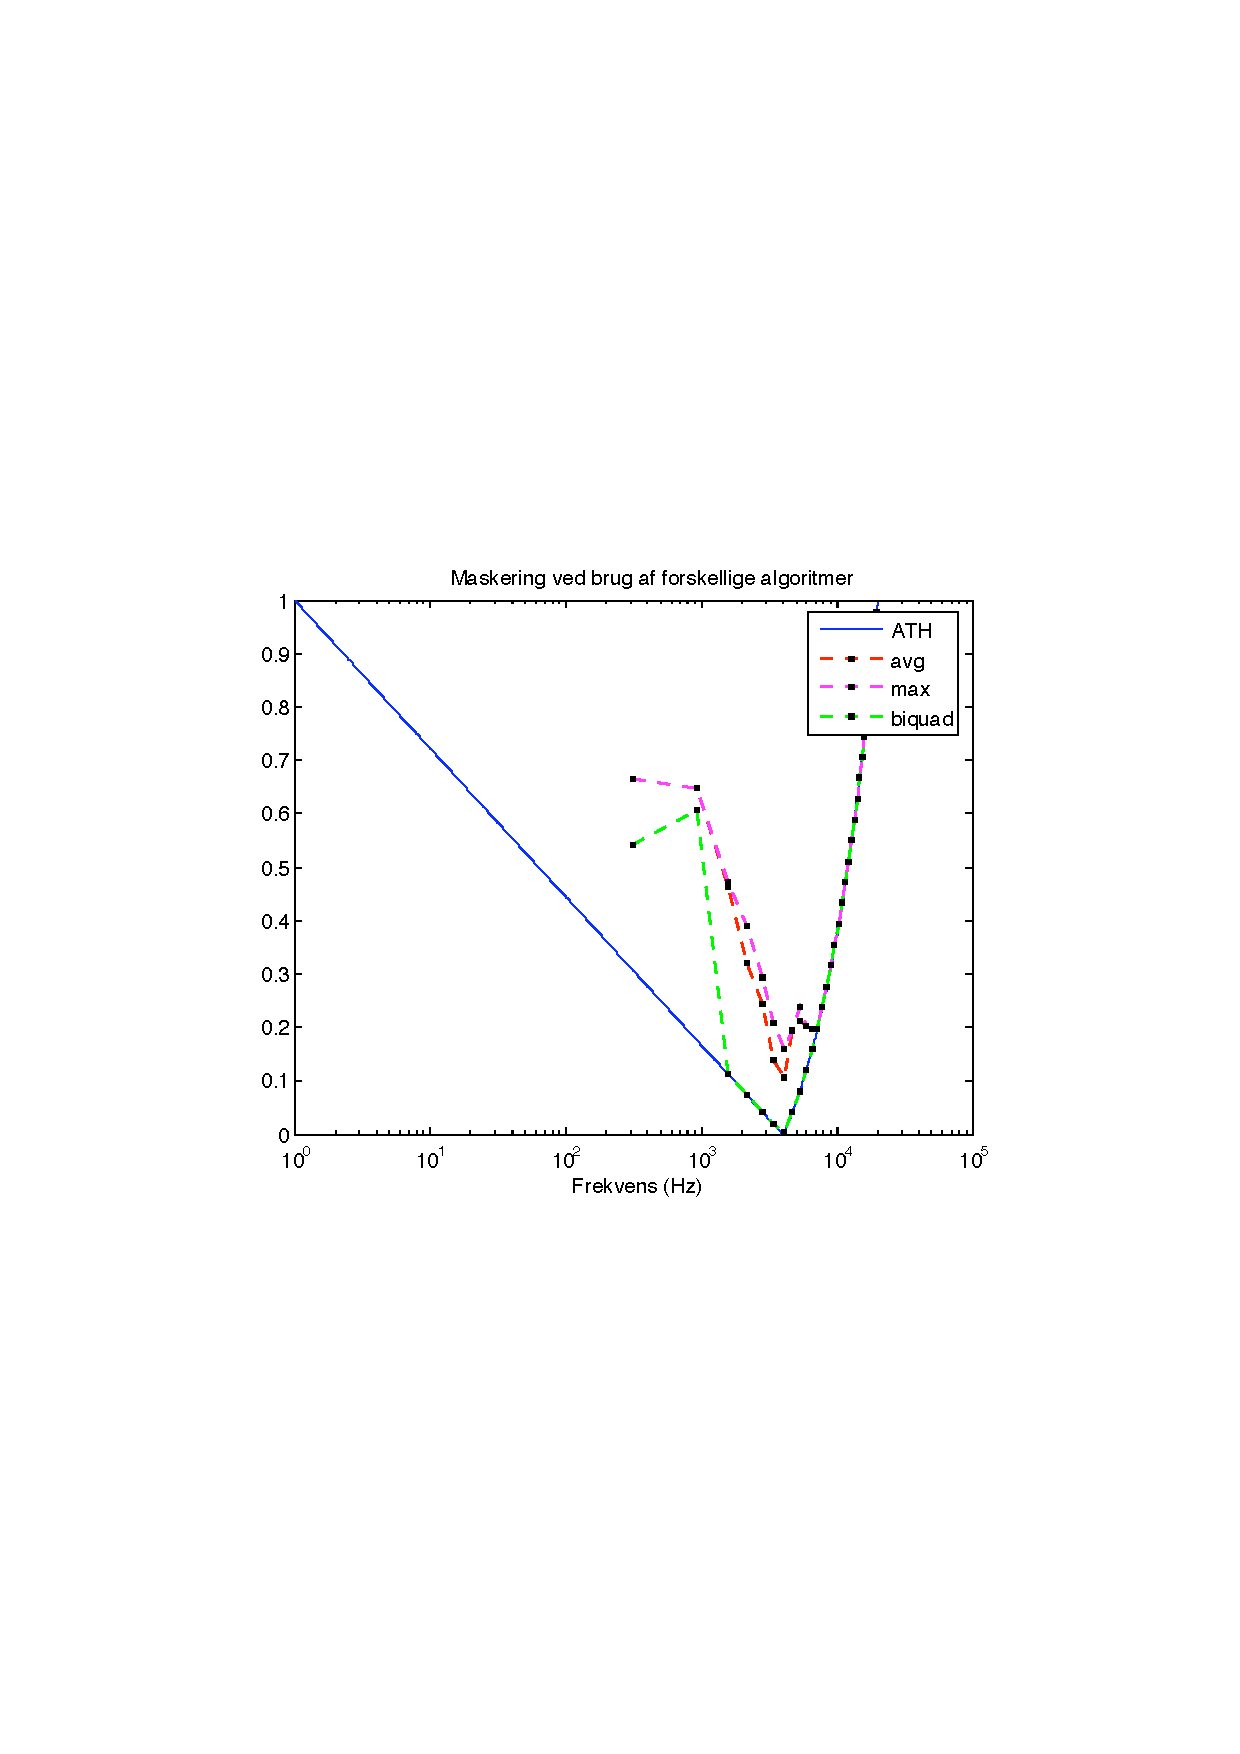
\includegraphics[width=12cm]{mask}
\end{center}
\caption{De forskellige maskeringsteknikker}
\label{fig.mask}
\end{figure}


\subsection*{maxmask og avgmask}
Initielt har vi lavet to enkle modeller, hvor et frekvensbånd
maskeres, hvis det naboer er tilstrækkeligt kraftige.\\
Det ene baseres på den maksimale værdi af de to naboer og den anden på
gennemsnittet. Begge modeller har det problem at de ikke kan se mere
end 1 bånd væk, men dette vil blot introducere områder hvor yderligere
optimering kunne foretages og vil derfor producere et output som
mindre optimeret men ikke med forringet lydkvalitet.

\subsection*{Biquad-maskering}
De tidligere beskrevne maskeringsmetoder benytter sig kun af
informationer fra de to omkringliggende bånd. Biquad maskering er et
forsøg på at lave alle bånd kunne maskere hinanden, uden at de ved et
uheld kommer til at maskere sig selv.\\
Maskeringskurven er frembragt på følgende vis:
\begin{itemize}
\item Der genereres en blok med hvidstøj.
\item For hver bånd maxværdi som ligger over ath-kurven, lav en parametrisk
  equalisering af hvidstøjen, hvor gain er styret af signal-to-ath
  ratio og båndbredden er fikseret til 1/2 oktav. Dette gøres ikke for
  båndet selv, idet det således ville kunne overkygge sig selv.
\item FFT af signalet, så vi kommer tilbage i frekvensdomænet
\item Smooth grafen
\item Lav maskeringsopslaget for det givne bånd.
\end{itemize}
Dette gøres dynamisk for hver frame, bortset fra
hvidstøjsgenereringen. Den laves kun een gang og genbruges derefter.

